%! Author = Dean
%! Date = 12/30/2023

\chapter{Komponente konvolucijskih neuronskih mreža}\label{ch:komponente-konvolucijskih-neuronskih-mreza}
Konvolucijske neuronske mreže, baš kao i obične neuronske mreže, sastoje se od ulaznog sloja, izlaznog sloja i skrivenih slojeva.
U matematičkom smislu, konvolucija predstavlja proces kombiniranja dviju funkcija kako bi se generirala treća funkcija poznata kao izlazna funkcija.

\section{Konvolucijski sloj}\label{sec:konvolucijski-sloj}
Jedan od glavnih gradivnih blokova konvolucijske neuronske mreže je konvolucijski sloj.
Sloj se sastoji od ulaznih vektora, izlaznih vektora ili mapa značajki i sastoji se od filtra ili kernela.
Filtri su uglavnom male matrice veličine 3x3, 5x5 ili 1x1, a sami filtri služe da izvuču bitne informacije \emph{značajke} iz ulaznih vektora.
Iz tog razloga nećemo imati samo jedan filtar, jer s jednim filtrom ne možemo izvući sve potrebne značajke.
Filtar se primjenjuje na ulazne podatke tako što pomnoži elemente na istim pozicijama i sumira njihove vrijednosti.
Taj proces je poznat kao konvolucija.

\FloatBarrier
\begin{figure}[h]
    \centering
    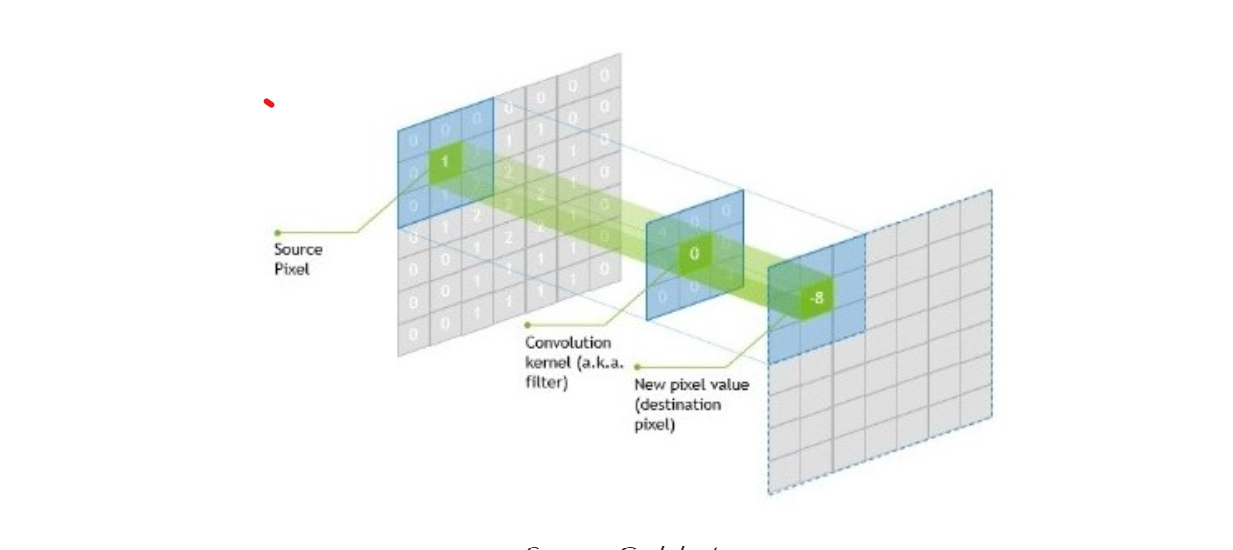
\includegraphics[width=0.7\textwidth]{images/Convolution}
    \caption{Konvolucijski sloj
    \protect\footnotemark}
    \label{fig:slika13}
\end{figure}
\FloatBarrier

\footnotetext{\url{https://www.analyticsvidhya.com/blog/2022/03/basics-of-cnn-in-deep-learning/}}

U konvolucijskom sloju koristimo nadopunjavanje \emph{padding} i korak \emph{stride}, a oni zapravo određuju kako će se prevesti konvolucija ulaznih podataka i dimenzija izlaza.
Za njih možemo reći da su hiperparametri.

Korak nam govori kako filtar primjenjujemo na ulaznu matricu, odnosno kako se krećemo po matrici po stupcima.
Ako postavimo korak na 1, filtar će se pomaknuti za 1 stupac u lijevo do kraja, dok će se s korakom 2 pomaknuti za 2 stupca.
Jasno je da veći korak rezultira manjom dimenzijom izlaza, i obrnuto.
\FloatBarrier
\begin{figure}[h]
    \centering
    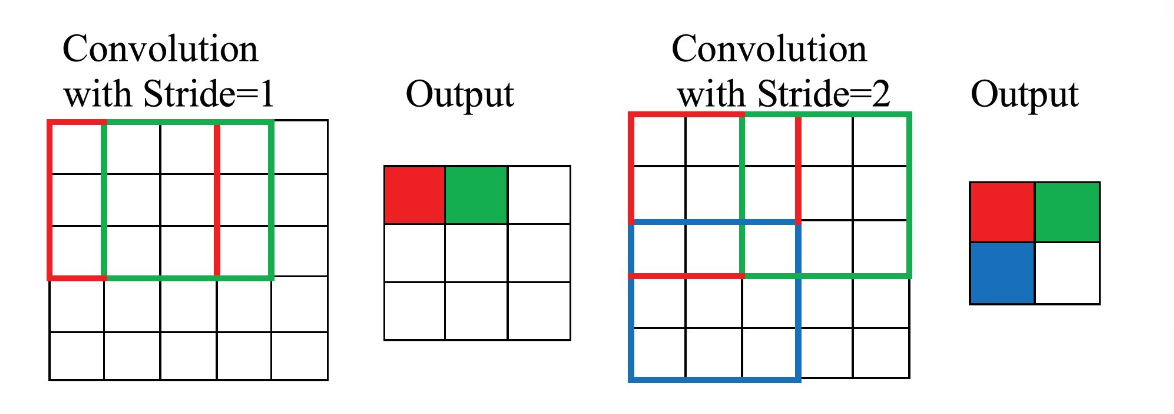
\includegraphics[width=0.7\textwidth]{images/Stride}
    \caption{Učinak različitih vrijednosti koraka \emph{stride}
    \protect\footnotemark}
    \label{fig:slika14}
\end{figure}
\FloatBarrier
\footnotetext{\url{https://www.analyticsvidhya.com/blog/2022/03/basics-of-cnn-in-deep-learning/}}


Problem je što na ovaj način možemo izgubiti potrebne informacije, a i informacije koje se nalaze na samom rubu i u kutovima se puno manje koriste.
Zbog toga imamo takozvani \enquote{padding}, što je zapravo proces nadopunjavanja ulazne matrice.
Postoje dvije tehnike nadopunjavanja: bez nadopunjavanja (\emph{valid padding}) i nadopunjavanje istom količinom (\emph{same padding}).
Kod tehnike \emph{valid padding}, zapravo ne radimo ništa i dozvoljavamo da se dimenzija izlaza smanji, dok kod \emph{same padding} tehnike dodajemo dodatne retke i stupce, popunjene nulama, kako bismo očuvali dimenziju izlaza i dali više značaja originalnim rubnim pozicijama.

\FloatBarrier
\begin{figure}[h]
    \centering
    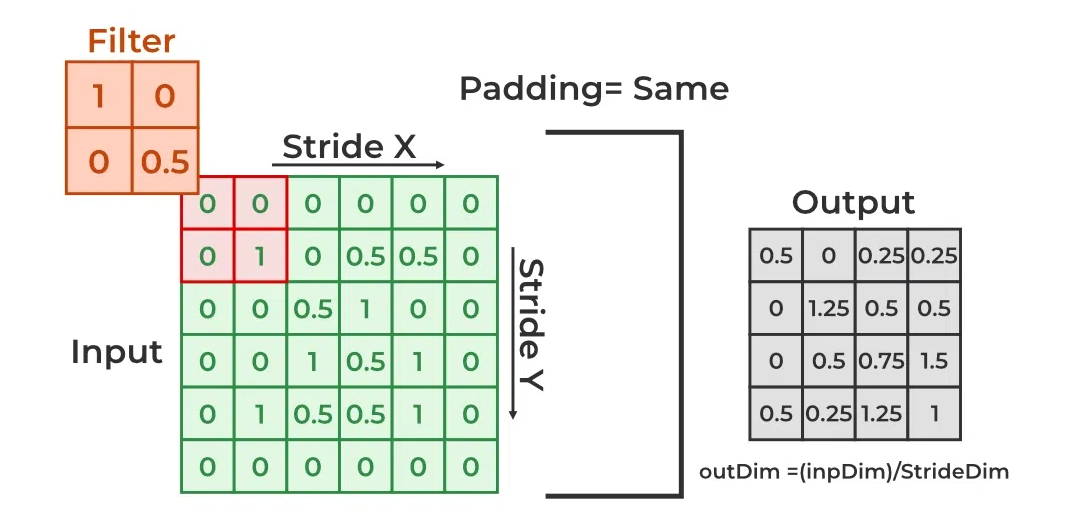
\includegraphics[width=0.6\textwidth]{images/Padding}
    \caption{Učinak nadopunjavanja \emph{same padding}
    \protect\footnotemark}
    \label{fig:slika15}
\end{figure}
\FloatBarrier
\footnotetext{\url{https://www.geeksforgeeks.org/cnn-introduction-to-padding/}}


\section{Sloj uzrokovanja}\label{sec:sloj-uzrokovanja}
Uloga ovog sloja je postupno smanjiti dimenzije svake značajke, odnosno izlaza konvolucijskog sloja, i na taj način smanjiti broj parametara.
Obično se sloj za uzrokovanje radi s matricom 2x2.

\FloatBarrier
\begin{figure}[h]
    \centering
    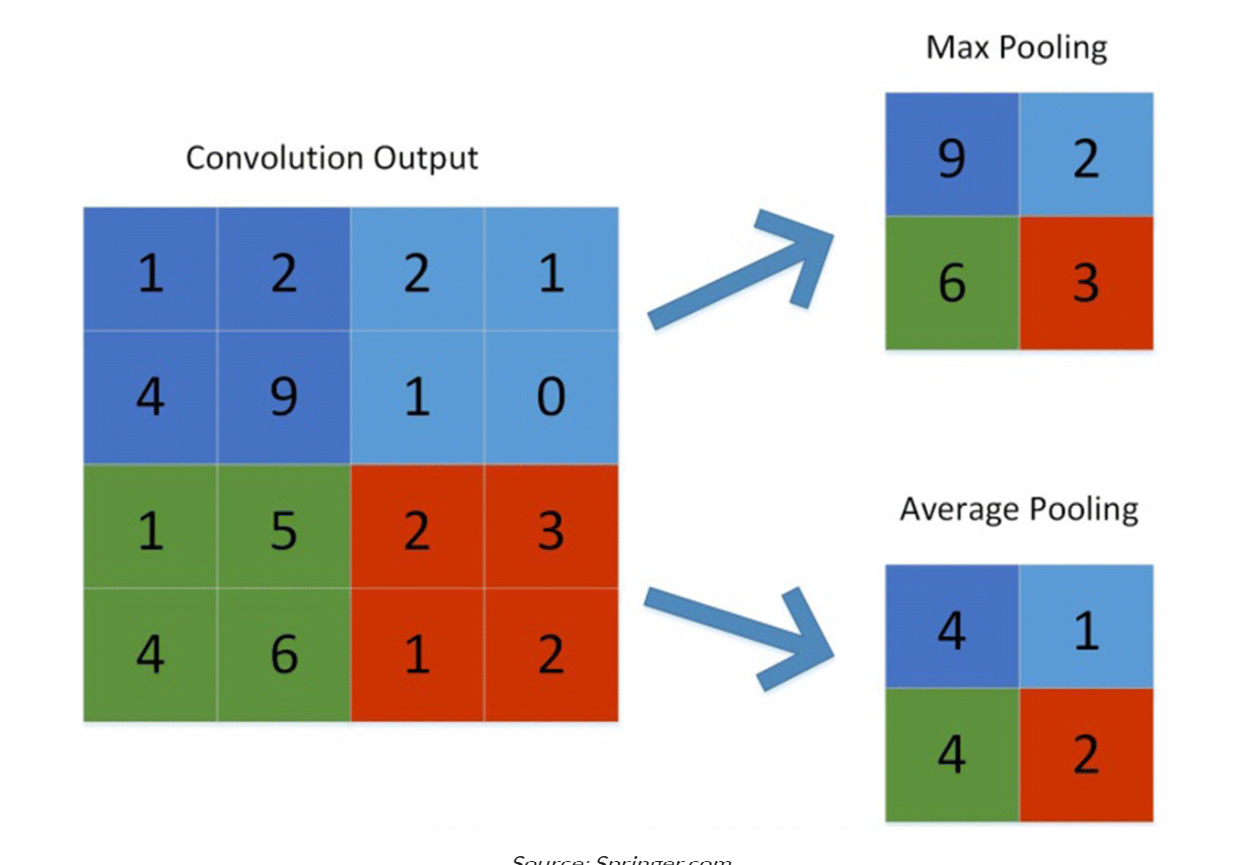
\includegraphics[width=0.7\textwidth]{images/Pooling}
    \caption{Prikaz \emph{max padding-a} i \emph{average padding-a}
    \protect\footnotemark}
    \label{fig:slika16}
\end{figure}
\FloatBarrier
\footnotetext{\url{https://www.geeksforgeeks.org/cnn-introduction-to-padding/}}


Postoje dvije metode za uzrokovanje: \emph{average pooling} metoda računa prosjek elemenata u matrici, dok \emph{max pooling} metoda, češće korištena, uzima element s najvećom vrijednošću.
Što je veća matrica za uzrokovanje, to će dimenzije biti manje, i obrnuto.

\section{Potpuno povezani sloj}\label{sec:potpuno-povezani-sloj}
Potpuno povezani sloj zapravo je unaprijedna neuronska mreža.
Njezin ulaz je izlaz konvolucijskog sloja ili sloja za uzrokovanje, a kako bismo te izlaze mogli unijeti kao ulaz u neuronsku mrežu, prvo moramo matricu pretvoriti u vektor.
Nakon toga imamo niz skrivenih slojeva u neuronskoj mreži, a na kraju imamo izlazni sloj koji će dati rezultat cijelog ovog procesa.